
\documentclass{beamer}

\usepackage[utf8]{inputenc}
\usepackage[spanish]{babel}
\usepackage{verbatim}

\usepackage{beamerthemesplit}

\usetheme{Warsaw} 

\title{Proxy POP3}
\subtitle{Castiglione, Galindo, Karpovsky}
\author{Protocolos de Comunicación\\  ITBA}
\date{Miércoles 31 de Octubre}



\begin{document}

\frame{\titlepage}

\begin{frame}[allowframebreaks]{Tabla de contenidos}
\tableofcontents
\end{frame}

\section{Introducción}
\subsection{RFCs relevantes}
\begin{frame}{RFCs relevantes}
\begin{itemize}
    \item \textbf{RFC 1939:} Post Office Protocol - Versión 3
    \item \textbf{RFC 2045, 2046, 2047:} Multipurpose Internet Mail Extensions
    \item \textbf{RFC 822:} Standard for the format ofarpa internet text messages
    \item \textbf{RFC 2119:} Key words for use in RFCs to Indicate Requirement Levels
\end{itemize}
\end{frame}

\subsection{Librerías a utilizar}
\begin{frame}{Librerías a utilizar}
\begin{itemize}
    \item \textbf{Log4j:} Logueo de informacion.
    \item \textbf{JodaTime:} Manejo de fechas.
    \item \textbf{Java.Util.Concurrent:} Manejo de concurrencia.
    \item \textbf{java.nio.file:} Monitoreo por cambios de directorios.
\end{itemize} 
\end{frame}

\section{POP3 Proxy}
\subsection{Arquitectura general}
\begin{frame}{Arquitectura general}
\begin{figure}[H]
\begin{center}
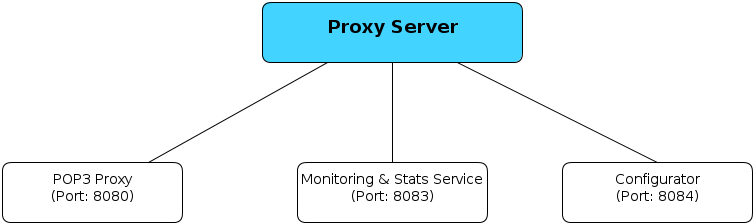
\includegraphics[scale=0.40]{./images/Servers.png}
\label{modelado}
\end{center}
\end{figure}
\end{frame}

\begin{frame}{Servicios}

\par \textbf{Servicio de monitoreo (8081):} El servicio de monitoreo sirve para poder visualizar, de manera remota, las estadísticas generales del servidor proxy. Basta con conectarse al puerto 8083 del servidor e ingresar la clave de administrador para la sección de monitoreo. Ejemplo de conexión al servicio de monitoreo:

\begin{block}{Conexión por netcat al servicio de monitoreo}
nc localhost 8081
\end{block}

\par \textbf{Servicio de configuración remota (8082):} El servicio de configuración remota escuchará en el puerto 8084. En secciones posteriores se detalla el funcionamiento de este servicio.

\end{frame}

\begin{frame}{Arquitectura general: Servicios}
\begin{figure}[H]
\begin{center}
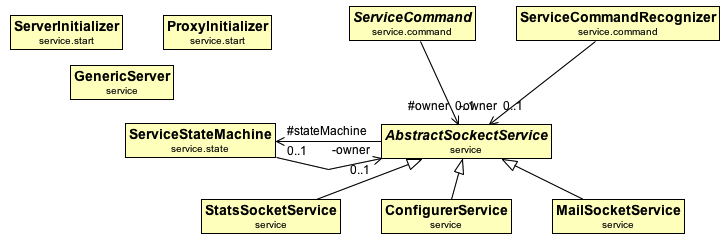
\includegraphics[scale=0.45]{./images/SocketService.png}
\label{modelado}
\end{center}
\end{figure}
\end{frame}

\section{Configuración de la aplicación}
\begin{frame}{Configuración de la aplicación}

\par La configuración del proxy se hará por medio de archivos que se escanearán permanentemente para detectar cambios en ellos.\\[1cm]
\par Por ejemplo, si que quieren agregar los filtros de ip, bastará con crear un archivo \textit{bannedips.conf}, y copiarlo al directorio \textit{/config/filters/bannedips.conf}.

\end{frame}

\subsection{Archivos de configuración}

\begin{frame}{origin\textunderscore server.conf}

\par Sirve para configurar un origin server distinto del default: se requiere la dirección del origin server deseado y el puerto. A través de este archivo se podría hacer el encadenamiento de proxys\\[0.5cm]

\begin{block}{Formato del archivo de configuración}
dest = mail.itba.edu.ar\\
port = 110\\
\end{block}


\end{frame}

\begin{frame}{monitor.conf}

\par Define todas las opciones de configuración referentes al servicio de estadísticas y monitoreo remoto que corre en el puerto 8083\\[0.5cm]

\begin{block}{Formato del archivo de configuración}
password = secreta\\
refresh\textunderscore rate\textunderscore ms = 2000

\end{block}

\end{frame}

\begin{frame}{transformations.conf}

\par Contendrá la lista de todas las modificaciones que se le deban aplicar a los mensajes de correo electrónico. Las transformaciones funcionan de manera global (no por usuario). Es decir, si se activa \textit{l33t}, todos los mensajes que el servidor proxy forwardee a los MUA vendrán modificados con la estrategia \textit{l33t}\\[0.5cm]

\begin{block}{Formato del archivo de configuración}
l33t\\
rotateImages\\
hideSender\\
\end{block}

\end{frame}

\begin{frame}{access\textunderscore time.conf}

\par Aquí se define el control de accesos por rangos horarios para cada uno de los usuarios\\[0.5cm]

\begin{block}{Formato del archivo de configuración}
juan@zauberlabs.com = 9:00-11:00\\
juan@monits.com = 19:00-22:00\\
\end{block}

\end{frame}

\begin{frame}{access\textunderscore ip.conf}

\par Aquí se define el control de accesos por dirección IP \\[0.5cm]

\begin{block}{Formato del archivo de configuración}
200.232.11.89\\
74.232.111.0/24\\
88.1.13.0/16\\
\end{block}

\par Notar que la configuración permite bannear subredes.

\end{frame}

\begin{frame}{access\textunderscore count.conf}

\par Aquí se define el control de accesos por cantidad de logins exitosos. Los pares son del tipo [usuario, cantidad de logins admitidos por día]\\[0.5cm]

\begin{block}{Formato del archivo de configuración}
juan@hotmail.com = 9\\
pepe@gmail.com = 2\\
jorge@yahoo.com = 4\\
\end{block}

\end{frame}

\begin{frame}{dest\textunderscore servers.conf}

\par Este archivo permite lograr que para un determinado usuario no se utilice el mail server default\\[0.5cm]

\begin{block}{Formato del archivo de configuración}
juan@gmail.com = pop3.alu.itba.edu.ar\\
raul@gmail.com = pop3.other.server.com\\
\end{block}

\end{frame}

\begin{frame}{notdelete\textunderscore maxage.conf}

\par Aquí se pondrán reglas para la eliminación condicional por antiguedad. Sólo se permitirá borrar un mail si la fecha es mayor a la fecha delcarada en este archivo\\[0.5cm]

\begin{block}{Formato del archivo de configuración}
user@server.com = 15/02/2005\\
\end{block}

\end{frame}

\begin{frame}{notdelete\textunderscore sender.conf}

\par Los mensajes cuyo remitente sea alguno de los usuarios presentes en este archivo, no podrán ser borrados\\[0.5cm]

\begin{block}{Formato del archivo de configuración}
alan@gmail.com = usu1@hola.com, usu2@chau.com\\
jose@josegalindo.com.ar = karpoa@gmail.com\\
\end{block}

\end{frame}

\begin{frame}{notdelete\textunderscore header\textunderscore pattern.conf}

\par Sirve para definir borrados condicionales en base a headers que contengan los mensajes\\[0.5cm]

\begin{block}{Formato del archivo de configuración}
alan@gmail.com = MIME-Version eq 1.0, Content-Type eq text/plain\\
\end{block}

\end{frame}

\begin{frame}{notdelete\textunderscore contenttype.conf}

\par Sirve para definir borrados condicionales en base al tipo de archivos adjuntos\\[0.5cm]

\begin{block}{Formato del archivo de configuración}
alan@gmail.com = doc, pdf\\
juan@gmail.com = avi\\
\end{block}

\end{frame}

\begin{frame}{notdelete\textunderscore size.conf}

\par Sirve para definir borrados condicionales en base al tamaño del mensaje\\[0.5cm]

\begin{block}{Formato del archivo de configuración}
juan@gmail.com = 10000\\
alan@gmail.com = 100\\
\end{block}

\end{frame}

\begin{frame}{notdelete\textunderscore structure.conf}

\par Segun estructura del mensaje (Ejemplo: Mensajes con adjuntos)\\[0.5cm]

\begin{block}{Formato del archivo de configuración}
hasAttachments\\
\end{block}

\end{frame}

\section{Protocolos desarrollados: Configuración remota}

\begin{frame}{Protocolos desarrollados}

\par Para configurar el servidor de forma remota lo que se debe hacer es conectarse a un servicio que éste provee en el puerto \textbf{8084} y hablar el \textbf{Protocolo de Configuración Remota} definido en la siguiente sección.

\end{frame}

\subsection{Protocolo de Configuración Remota}

\begin{frame}{Protocolo de configuración remota}

\par El protocolo de configuración remota es del tipo \textit{request - response}, cada vez que el cliente ejecuta un comando, el servidor le responderá con \textbf{+OK} o \textbf{-ERR} en caso de una ejecución satisfactoria o una ejecución con errores respectivamente.

\end{frame}


\subsubsection{Ejecución satisfactoria}

\begin{frame}{Protocolo de configuración remota: Ejecución satisfactoria}

\par En el caso de una ejecución satisfactoria, el servidor enviará el mensaje \textbf{+OK} y el \textit{status code} 0. Se reservan los códigos de estado desde el 0 al 99 para respuestas relacionadas con ejecuciones correctas en futuras extensiones del protocolo.

\begin{block}{Ejecución satisfactoria}
+OK 0 [Message]
\end{block}

\end{frame}

\subsubsection{Ejecución con errores}

\begin{frame}{Protocolo de configuración remota: Ejecución con errores}

\par Los \textit{status code} del 100 en adelante están intencionados para casos en los que el servidor deba comunicar cualquier tipo de error. El servidor puede incluír una entidad conteniendo una explicación de la situación de error e informando si ésta es una situación permanente o temporaria.\\

\begin{alertblock}{Ejecución con errores}
-ERR ERROR\textunderscore CODE [HUMAN READABLE ERROR MESSAGE]
\end{alertblock}


\par Los programas externos que implementen este protocolo podrían mostrarle al usuario cualquier entidad incluída junto a los códigos de error con el fin de ser más amigables para con el usuario.\\

\end{frame}

\begin{frame}{Protocolo de configuración remota: Ejecución con errores}

\begin{tabular}{|l|l|}
  \hline
  \multicolumn{2}{|c|}{Error codes} \\
  \hline
  \hline
  100 & Unrecognized command \\
  101 & Invalid parameters: missing arguments \\
  102 & Invalid parameters: file does not exists \\
  103 & Invalid parameters: unrecognized user \\
  104 & Invalid parameters: not a number \\
  111 & Invalid password \\
  \hline
\end{tabular}
\end{frame}


\subsection{Comandos soportados}

\begin{frame}{Comandos soportados}
\par El servicio de configuración soporta los comandos: \textbf{AUTH}, \textbf{LIST}, \textbf{GET}, \textbf{PUT}, \textbf{DEL}, \textbf{EXIT}. A continuación se explicará en detalle el funcionamiento de cada uno de ellos.

\end{frame}


\subsubsection{AUTH password}
\begin{frame}{Comandos soportados: AUTH password}

\par El método \textbf{AUTH} sirve para autenticarse contra el servidor de configuración. Recibe como único parámetro la contraseña con la cual el cliente que se quiere autenticar.\\[0.5cm]
Posibles códigos de estado relacionados con el método \textbf{AUTH}: 0, 200
\end{frame}

\subsubsection{LIST}

\begin{frame}{Comandos soportados: LIST}

\par El método \textbf{LIST} imprime una lista de todos los comandos soportados por el servidor. No recibe parámetros. Es importante destacar que se impone como fin del mensaje una línea conteniendo únicamente el caracter punto (ASCII period).\\[0.5cm]
Posibles códigos de estado relacionados con el método \textbf{LIST}: 0, 100
Requiere estar autenticado para poder utilizarlo.
\end{frame}

\subsubsection{GET filename.conf}

\begin{frame}{Comandos soportados: GET fileName.conf}

\par El método \textbf{GET} recibe como único parámetro un string que contiene el nombre de un archivo de configuración e imprime el contenido de éste. Al igual que el método \textit{LIST}, utiliza el caracter punto para avisar el fin de su ejecución.\\[0.5cm]
Posibles códigos de estado relacionados con el método \textbf{GET}: 0, 100, 101, 102
Requiere estar autenticado para poder utilizarlo.
\end{frame}

\subsubsection{PUT filename.conf string}

\begin{frame}{Comandos soportados: PUT fileName.conf string}

\par El método \textbf{PUT} recibe dos parámetros: el nombre de un archivo de configuración y un \textit{string} en este órden. Lo que hace es agregar el \textit{string} recibido como parámetro en una nueva línea al final del archivo de configuración.\\[0.5cm]
Posibles códigos de estado relacionados con el método \textbf{PUT}: 0, 100, 101, 102
Requiere estar autenticado para poder utilizarlo.
\end{frame}

\subsubsection{DEL N filename.conf}

\begin{frame}{Comandos soportados: DEL N}

\par El método \textbf{DEL} rebice un número entero $N$ y el nombre de un arcvhivo de configuración. Su función es eliminar la línea $N$ del archivo en cuestión. \\[0.5cm]
 Posibles códigos de estado relacionados con el método \textbf{DEL}: 0, 100, 101, 102
 Requiere estar autenticado para poder utilizarlo.
\end{frame}

\subsubsection{EXIT}

\begin{frame}{Comandos soportados: EXIT}

\par El método \textbf{EXIT} varía su semántica según el usuario esté o no esté autenticado en el servidor de configuración: En caso de estar autenticado, el comando \textbf{EXIT} cierra la sesión; caso contrario, cierra la conexión con el servidor.\\[0.5cm]
Posibles códigos de estado relacionados con el método \textbf{EXIT}: 0
\end{frame}

\subsection{Ejemplo de configuración remota}
\begin{frame}{Ejemplo de configuración remota}
\par A continuación se presenta un ejemplo de configuración remota del servidor en el que el cliente es \textit{kickeado} por ingresar su contraseña de manera errónea 3 veces seguidas:

\end{frame}

\begin{frame}[fragile]{Ejemplo de configuración remota}
\begin{block}{}
S: +OK 0 [Server ready]\\
C: AUTH myUltraSecretPass\\
S: -ERR 200 [Invalid password]\\
C: AUTH anothedPassword\\
S: -ERR 200 [Invalid password]\\
C: AUTH forgottenPassword\\
S: -ERR 103 [Too many login attempts, try later.]
\end{block}
\end{frame}

\begin{frame}{Ejemplo de configuración remota}
\begin{columns}
\begin{column}{5cm}
\begin{block}{}
\scriptsize
S: +OK 0 [Server ready]\\
C: AUTH myPassword\\
S: +OK 0 [Password accepted]\\
C: LIST\\
S: ADD\\
S: DEL\\
S: AUTH\\
S: LIST\\
S: PRT\\
S: EXIT\\
S: .  // Period marks end of transmission\\
S: +OK 0 [Command listed]\\
C: PRT access\textunderscore ip.conf\\
S: 167.12.3.6\\
S: 162.11.23.5\\
S: .\\
S: +OK 0 [File access\textunderscore ip.conf printed]\\
\end{block}
\end{column}
\begin{column}{5cm}
\begin{block}{}
\scriptsize
C: ADD access\textunderscore ip 200.232.1.45\\
S: -ERR 102 [Configuration file not found]\\
C: ADD access\textunderscore ip.conf 200.232.1.45\\
S: +OK 0 [File access\textunderscore ip.conf updated]\\
S: 167.12.3.6\\
S: 162.11.23.5\\
S: 200.232.1.45\\
S: .\\
S: +OK 0 [File access\textunderscore ip.conf printed]\\
C: EXIT\\
S: +OK 0 [Good bye]\\
C: EXIT\\
S: +OK 0 [Good bye] // Connection clossed\\
\end{block}
\end{column}
\end{columns}
\end{frame}

\section{Problemas y dificultades detectados}
\subsection{Servicio y protocolo de configuración}
\begin{frame}{Servicio y protocolo de configuración}
\par Para implentar el servicio y el protocolo de configuración, en un primer momento se pensó es ir por una configuración orientada a archivos. Esta solución, cuya ventaja era era su rápida implementación y simplicidad, trajo consigo un conjunto de problemas:\\
\begin{itemize}
\item Imposiblidad de generar un protocolo coherente que funcionara con usuarios no humanos
\item Imposibilidad para imprimir la configuración actual del proxy (ya que pasandole el archivo se pisaba los archivos de configuración anteriores sin siquiera poder consultar su previo valor)
\end{itemize}
\end{frame}

\subsection{Multiplexación de cuentas}
\begin{frame}{Multiplexación de cuentas}
\par El problema que surgió en este punto estuvo relacionado con la forma en que los MUAs se autentican son el servidor. \\[0.5cm]
\par Fue necesario cerrar el conexión que se tenía anteriormente y crear una nueva conexión al servidor origin del usuario en particular, si así el archivo de configuración de multiplexación de cuentas así lo indicaba.
\end{frame}

\subsection{Parser de mails MIME}
\begin{frame}{Parser MIME}
\par El problema fue plantear una implementación del parser sin tener en cuenta que las partes de MIME pueden estar anidadas. Al descubrir esto se tuvo que hacer una remplementación del algoritmo de parseo, que se volvió considerablemente más complejo.
\end{frame}



\section{Casos de prueba}

\subsubsection{Tests Unitarios}
\begin{frame}{Tests unitarios}
\par    Se implementaron tests unitarios tanto para componentes de baja granularidad de la aplicación, como son los validadores y los transformadores (ImageTransformer, LeetTransformer y AnonymTransformer), como para las clases del modelo, específicamente User, y Mail, que modelan un usuario y a un correo electrónico, respectivamente. 
\end{frame}

\subsubsection{Tests de Integración}
\begin{frame}{Tests de integración}
\par	La finalidad sea probar la funcionalidad entera de la aplicación, mediante la interacción del proxy con servidores mock \textbf{(MockitoServer)}. De esta manera se va a poder probar los distintos requerimientos solicitados y el comportamiendo del proxy, por medio de escenarios de prueba exitosos y no exitosos, pudiendo así también probar, mediante la utilización de herramientas de testeo como \textbf{JMeter} , la performace del proxy.
\end{frame}

\section{Arquitectura de la aplicación}

\subsection{Máquina de estados}
\begin{frame}{Máquina de estados}
\par Se pensó la implementación como una máquina de estados donde, lógicamente, cada estado puede habilitar la ejecución de otros estados.\\[0.5cm]
Esta estrategia fue útil al realizar la multiplexación de cuentas y a su vez nos permite tener un código simple, limpio y entendible a la hora de extender el desarrollo.
\end{frame}

\begin{frame}{Arquitectura general: Máquina de estados}
\begin{figure}[H]
\begin{center}
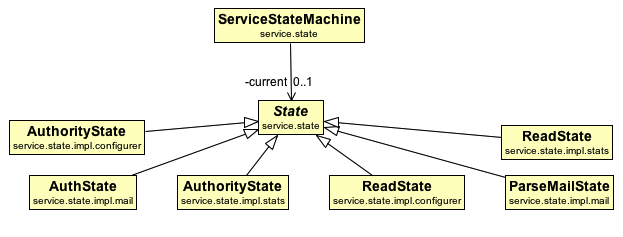
\includegraphics[scale=0.52]{./images/Estados.png}
\label{modelado}
\end{center}
\end{figure}
\end{frame}


\subsection{Control de accesos y validadores}

\begin{frame}{Arquitectura general: Control de accesos}
\begin{figure}[H]
\begin{center}
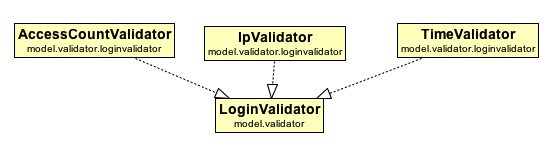
\includegraphics[scale=0.6]{./images/Validators.png}
\label{modelado}
\end{center}
\end{figure}
\end{frame}

\begin{frame}{Arquitectura general: Validadores de borrado}
\begin{figure}[H]
\begin{center}
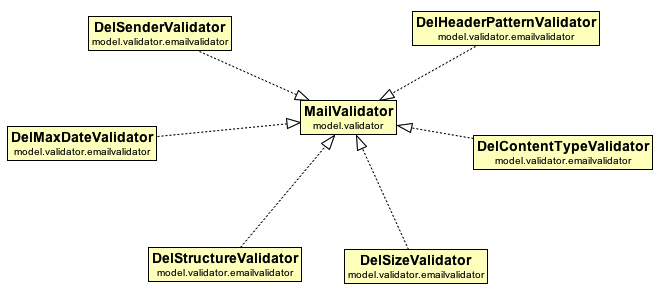
\includegraphics[scale=0.5]{./images/NotDelValidators.png}
\label{modelado}
\end{center}
\end{figure}
\end{frame}



\end{document}
